\chapter{
    \textbf{EXPERIMENTAL RESULTS}
}
\justifying{
    \large
        \paragraph{} Experiments were performed on standard test videos with colour frames. All the videos used have a resolution of 352 × 288, except Rhinos video which has a resolution of 320 × 240. Texts with different lengths were used as secret messages embedded in the test video files.\\
        \begin{figure}[h]
            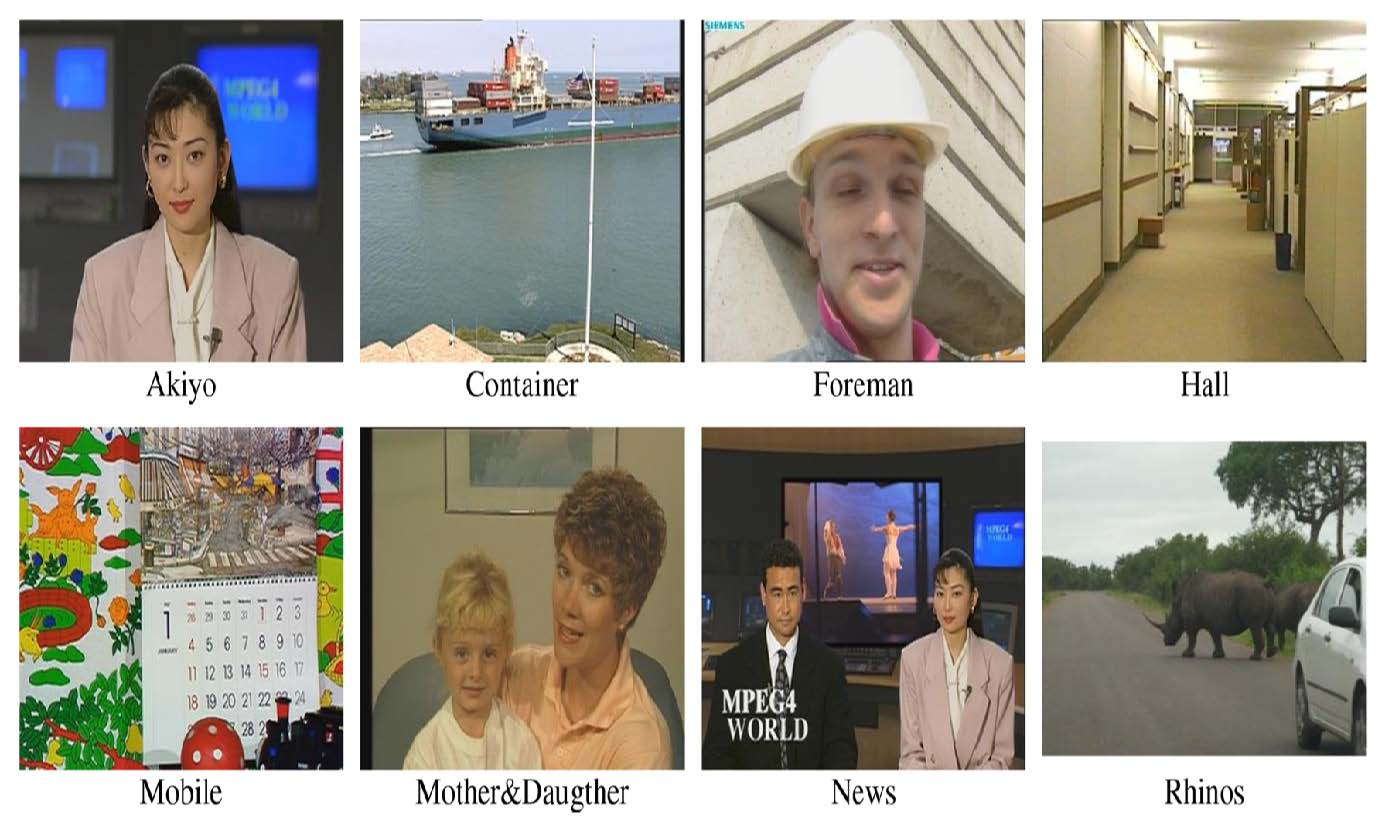
\includegraphics{images/6.jpg}
            \caption{Frame samples of standard test videos.}
        \end{figure}
}
\section{Performance Analysis}
\subsection{PSNR}
\justifying{
    \large
        \paragraph{} PSNR is used for the visual quality control of the stego videos. It is dependent on the variation of the mean square error (MSE) in the video frame. The less squared error and the higher PSNR mean the better the visual quality.
        \begin{figure}[h]
            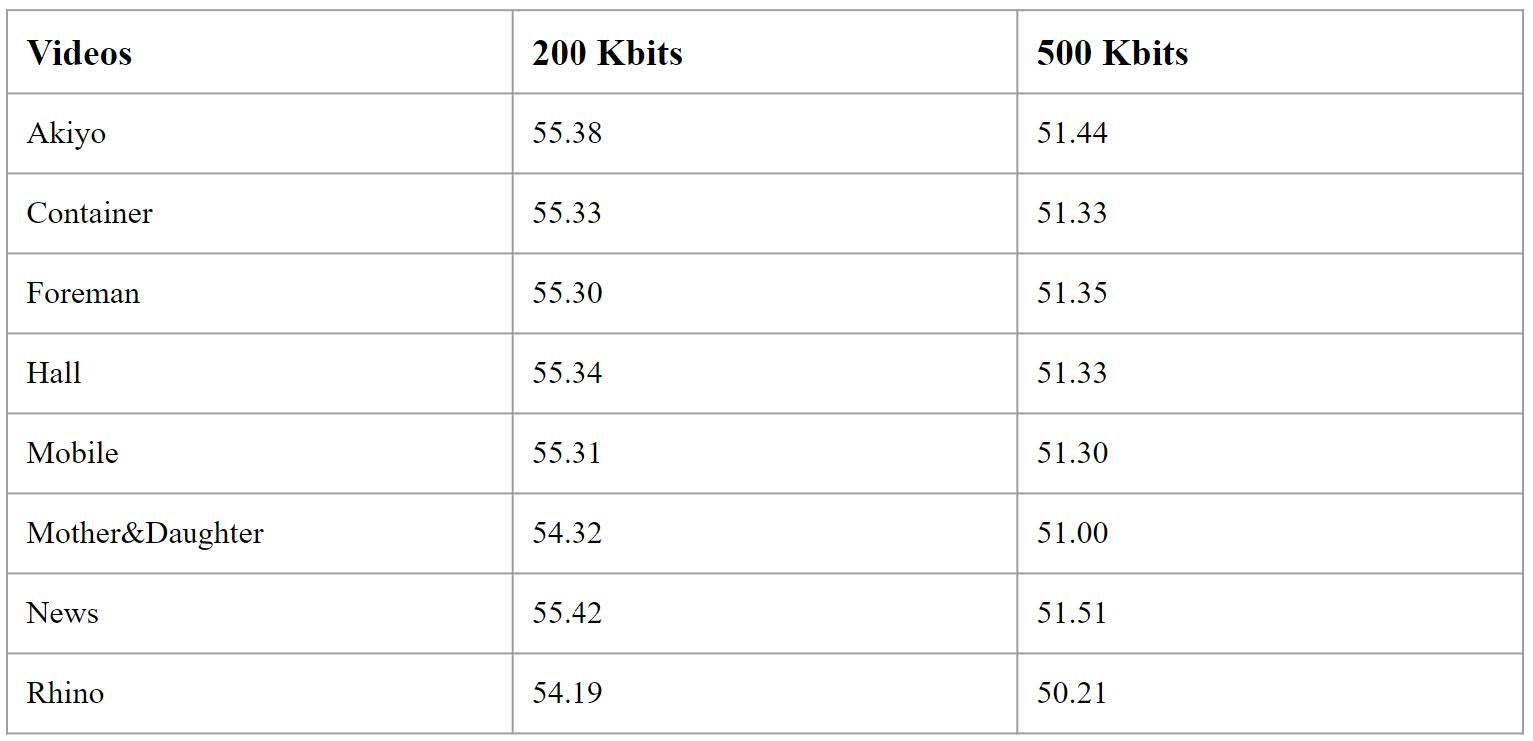
\includegraphics{images/7.jpg}
            \caption{PSNR (dB) values at 200 Kbits and 500 Kbits data capacity.}
        \end{figure}
        \paragraph{} The proposed method produced higher PSNR values (nearly 55 dB and 50 dB respectively) at 200 Kbits and 500 Kbits data hiding capacity than many of the existing data hiding methods.            
}
\subsection{SSIM}
\justifying{
    \large
        \paragraph{} SSIM is a quality criterion that looks at the similarity over luminance, contrast and structure components in video frames or images. When the similarity is highest, SSIM takes the value 1. With the decrease of similarity, SSIM value approaches zero.
        \begin{figure}[h]
            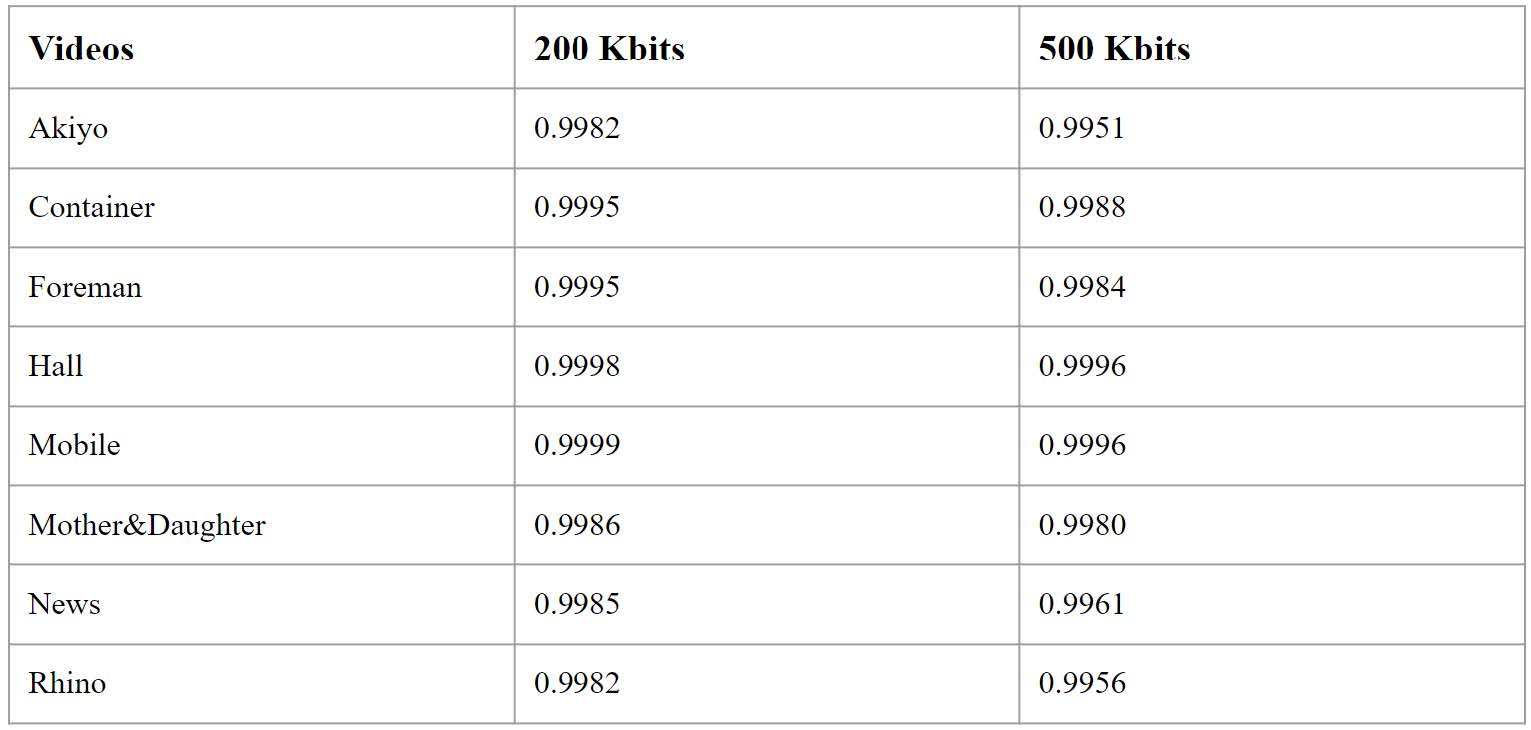
\includegraphics{images/8.jpg}
            \caption{SSIM values at 200 Kbits and 500 Kbits data capacity.}
        \end{figure}
        \paragraph{} It was observed that the SSIM values for the proposed method are very close to 1 and hence it is superior to other methods.            
}
\subsection{NCC}
\justifying{
    \large
        \paragraph{} In a good data hiding algorithm, the similarity ratio between the hidden message and the extracted message should be at the highest level. Normalised correlation coefficient (NCC) value is 1 if the secret message is exactly the same. The NCC value decreases as the losses in the message.
        \begin{figure}[h]
            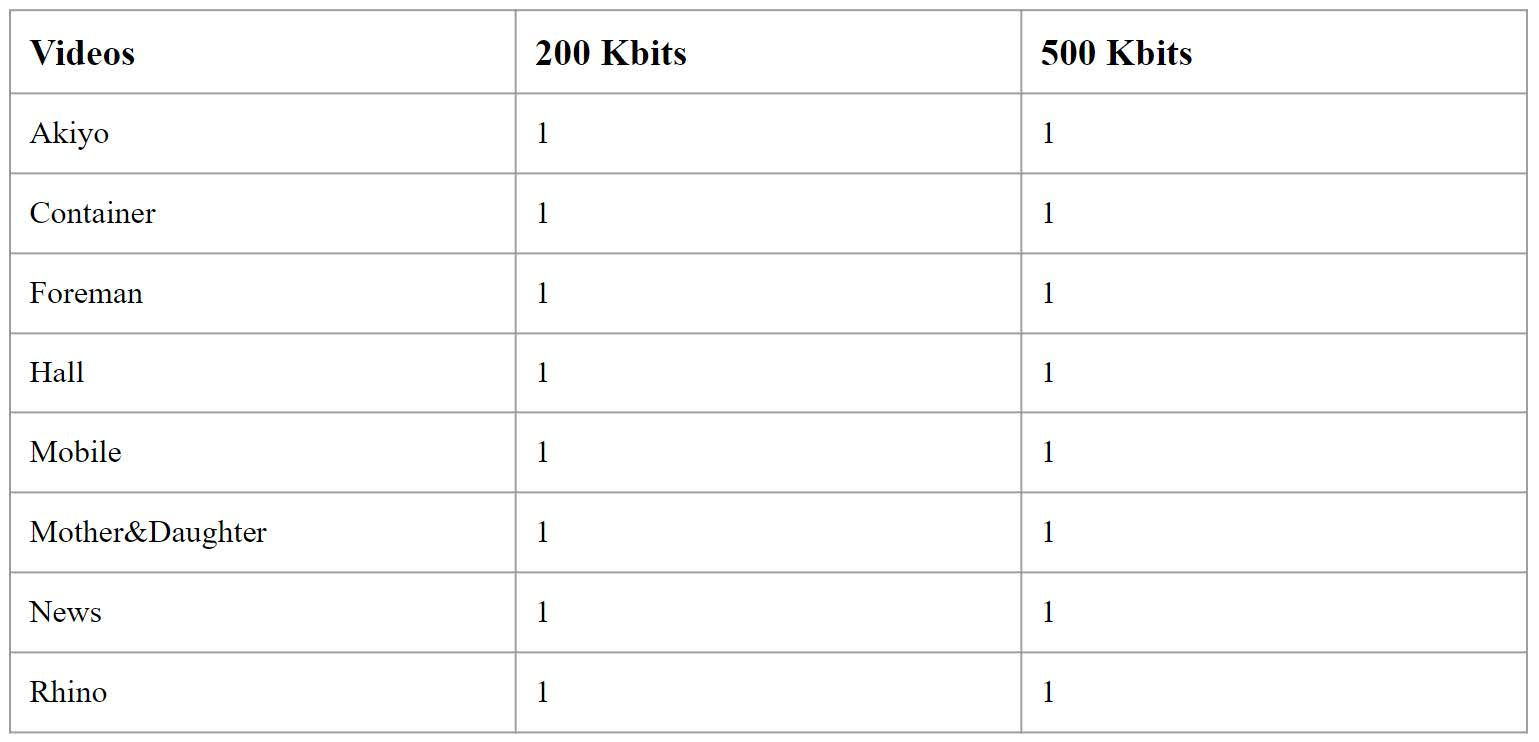
\includegraphics{images/9.jpg}
            \caption{NCC values at 200 Kbits and 500 Kbits data capacity.}
        \end{figure}
        \paragraph{} The NCC value for the different test videos of the proposed method is 1, therefore, the extracted message is exactly the same as the secret message.            
}
\subsection{BER}
\justifying{
    \large
        \paragraph{} The bit error rate (BER) value used to control the amount of error between embedded and extracted messages. The BER value indicates the distortion rate of the hidden message.
        \begin{figure}[h]
            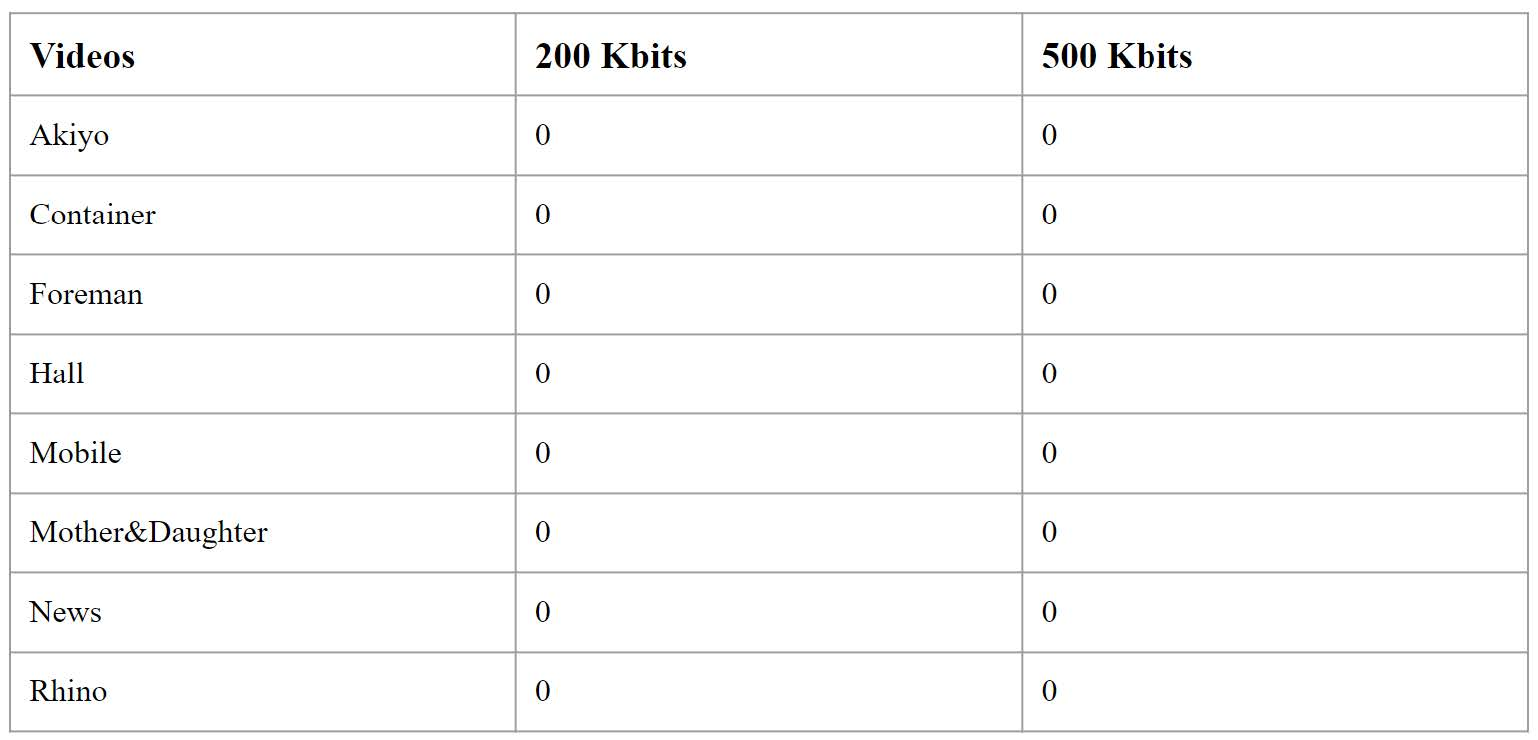
\includegraphics{images/10.jpg}
            \caption{BER values at 200 Kbits and 500 Kbits data capacity.}
        \end{figure}
        \paragraph{} The BER (\%) of the proposed method was found to be 0, indicating that there was no error between the hidden message and the extracted message.           
}
\section{Comparison with classical LSB332}
\justifying {
    \large
        \begin{figure}[h]
            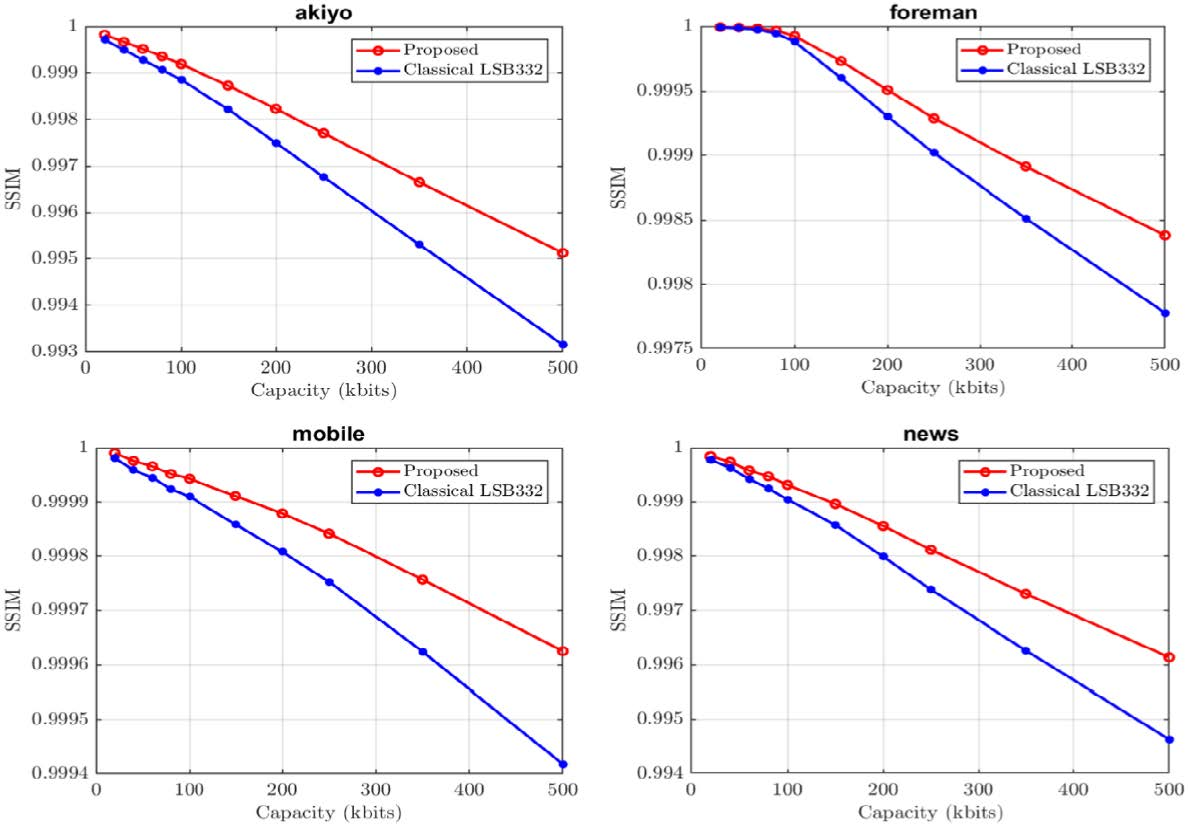
\includegraphics{images/11.jpg}
            \caption{SSIM values at different data capacities.}
        \end{figure}
        \paragraph{} From the above graph, it was observed that the proposed adaptive inverted LSB332 method produced higher SSIM values at increased data capacities than the classical LSB332 method.
        
}
\section{Steganalysis Attacks}
\subsection{Pixel Difference Histogram (PDH)}
\justifying {
    \large
        \paragraph{} PDH calculates the successive pixel differences and compares these distributions of the cover and stego video frames. If the curves overlap, the hidden data cannot be detected. When the figure \ref{fig:PDH} is examined, the curves of the cover and stego frames are found to be overlapping and hence, the proposed method is resistant to PDH attacks.
        
}
\subsection{Histogram Analysis}
\justifying {
    \large
        \paragraph{} Histogram analysis compares the pixel value distributions of cover video frame and stego video frame. Generally, comb effect is seen in LSB methods. When the figure \ref{fig:HA} is examined, no comb effect was observed in the stego frame because in the proposed method, the secret data is distributed to the selected video frames.
        
}
\begin{figure}[ht]
    \centering
    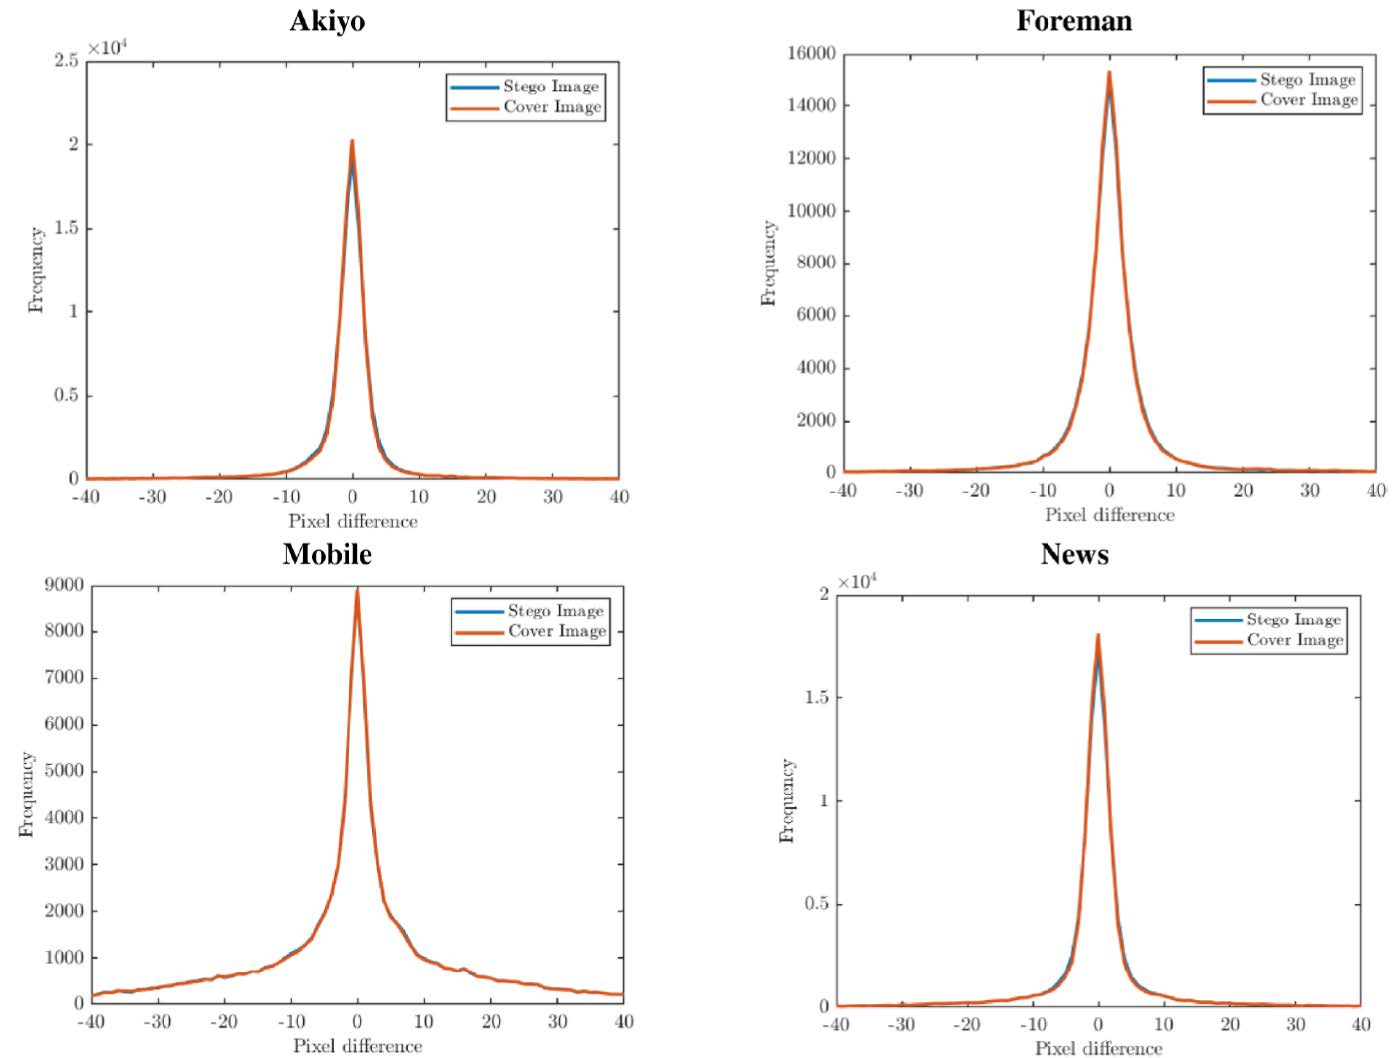
\includegraphics[scale=0.815]{images/12.jpg}
    \caption{Pixel difference histogram of the proposed method.}
    \label{fig:PDH}
\end{figure}
\begin{figure}[ht]
    \centering
    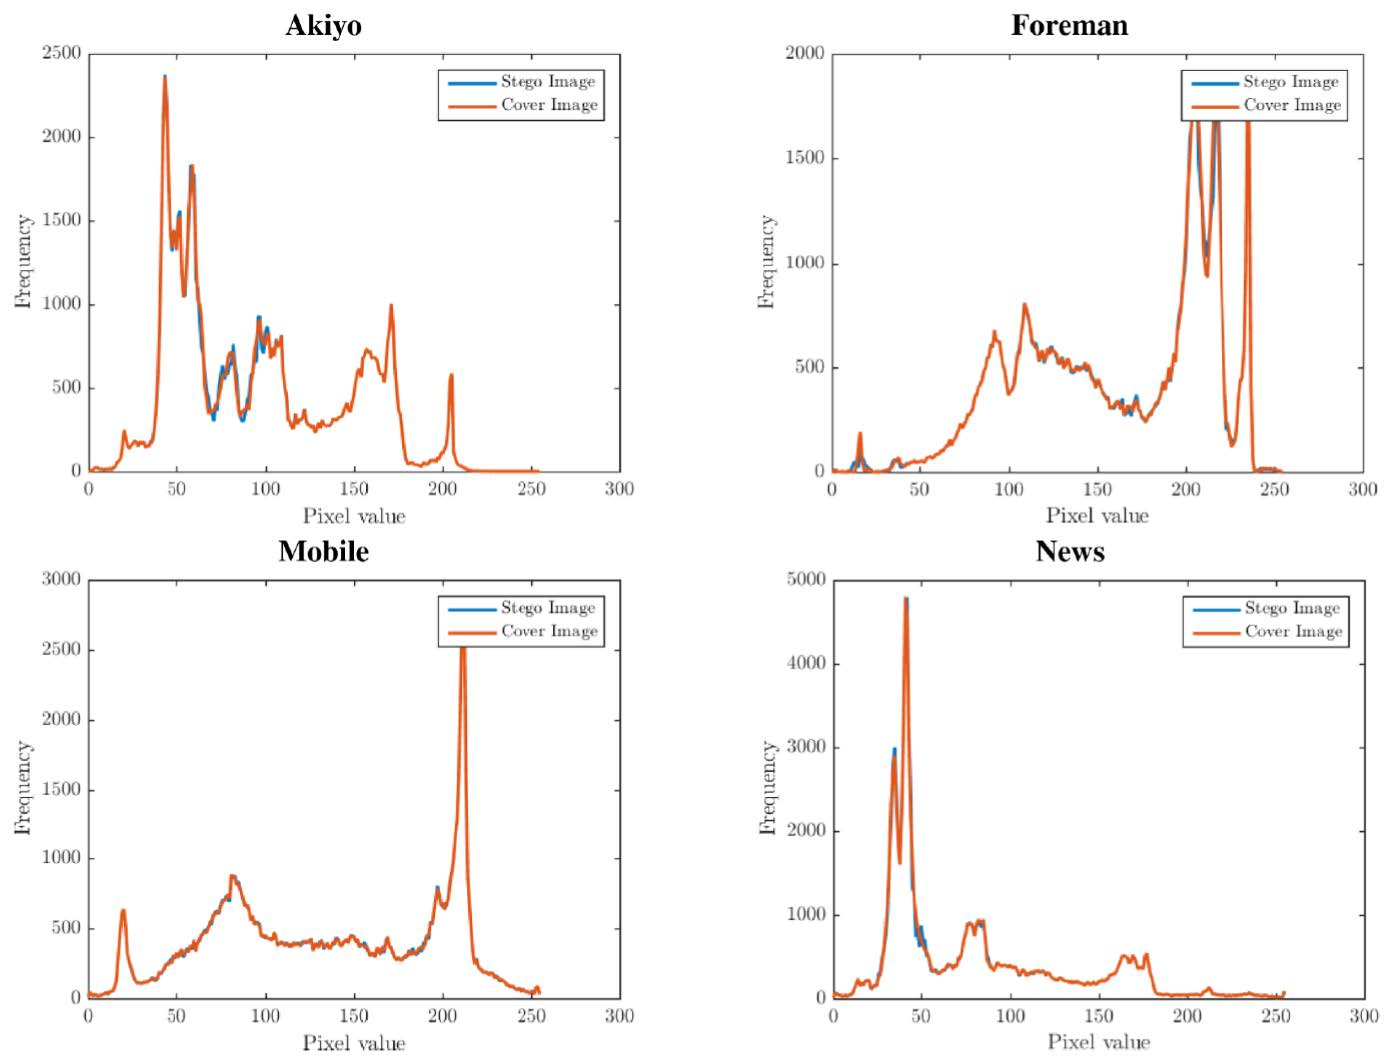
\includegraphics[scale=0.815]{images/13.jpg}
    \caption{Comparisons of histogram analysis of the proposed method.}
    \label{fig:HA}
\end{figure}
\subsection{Complexity analysis}
\justifying {
    \large
        \paragraph{} The computational complexity of the LSB-based algorithms in the literature is known as O(n). However, the computational complexity of the proposed data hiding algorithm was observed to be O(n2). In addition, O(n) computational complexity occurs during the Vigenere-based frame selection process. Therefore, the total computation complexity of the proposed algorithm is O(n + n2) that is realised as O(n2). Although the Vigenere-based frame selection process consumes extra time and increases computational complexity, it makes embedding secret data more secure than the sequential frame selection process.
        
}